\documentclass[12pt,a4paper]{article}
\usepackage[utf8]{inputenc}
\usepackage[T1]{fontenc}
\usepackage{geometry}
\usepackage{amsmath}
\usepackage{amsfonts}
\usepackage{subcaption}
\usepackage[labelfont=bf]{caption}
\usepackage{amssymb}
\usepackage{graphicx}
\usepackage{float}
\usepackage{cite}
\usepackage{url}
\usepackage{hyperref}
\usepackage{subfigure}
\usepackage{booktabs}
\usepackage{multirow}
\usepackage{algorithm}
\usepackage{algorithmic}
\usepackage{listings}
\usepackage{xcolor}

\geometry{margin=1in}

\title{Uso di tecniche di LLM per analizzare traiettorie turistiche e per suggerire la prossima attrazione turistica da visitare}

\author{
Simone Mattioli\\
Dipartimento di Informatica\\
Università di Verona\\
}
\date{\today}

\begin{document}

\maketitle

\begin{abstract}
Questo articolo presenta uno studio completo sull'utilizzo dei Large Language Models (LLM) per prevedere i modelli di mobilità umana nei contesti turistici urbani. Introduciamo LLM-Mob, un nuovo framework che sfrutta le capacità di comprensione del linguaggio naturale dei moderni LLM per prevedere i prossimi Punti di Interesse (POI) dei turisti in base ai loro modelli di visita storici. Il nostro approccio viene valutato sul dataset VeronaCard, che contiene dati turistici reali di Verona, Italia, relativi a diversi anni. Viene analizzato l'impatto di diversi tipi di informazioni contestuali sull'accuratezza della previsione, inclusi nomi di POI di base, coordinate geografiche e caratteristiche temporali. Il framework dimostra il potenziale degli LLM per comprendere complessi modelli spazio-temporali nella mobilità umana senza richiedere un'ingegnerizzazione approfondita delle caratteristiche o architetture specifiche per dominio. L'implementazione sostituisce i tradizionali modelli GPT di OpenAI con modelli open source ( come Llama 3.1 ), rendendo l'approccio più accessibile ed economico per scopi di ricerca.
\end{abstract}

\newpage

\section{Introduzione}

La previsione della mobilità umana si è affermata come un'area di ricerca cruciale, con applicazioni che spaziano dalla pianificazione urbana ai sistemi di trasporto, dai sistemi di raccomandazione alla salute pubblica. Gli approcci tradizionali alla previsione della mobilità si sono basati in larga misura su modelli statistici, algoritmi di apprendimento automatico e architetture di deep learning specificamente progettate per dati sequenziali. Tuttavia, i recenti progressi nei Large Language Model (LLM) hanno aperto nuove strade per comprendere e prevedere i modelli di comportamento umano attraverso capacità di elaborazione del linguaggio naturale.

La sfida fondamentale nella previsione della mobilità umana risiede nel catturare la complessa interazione tra fattori spaziali, temporali e comportamentali che influenzano le decisioni di movimento individuali. Gli approcci tradizionali di apprendimento automatico richiedono spesso un'ampia progettazione di feature e conoscenze specifiche del dominio per codificare efficacemente queste relazioni. Al contrario, i LLM possiedono capacità intrinseche di comprensione delle relazioni e dei modelli contestuali, che possono essere sfruttate per prevedere i modelli di mobilità attraverso informazioni contestuali e prompt attentamente progettati.

Questo articolo presenta un framework che sfrutta la potenza dei Large Language Model per la previsione della mobilità umana in contesti turistici. Il mio approccio si differenzia dai metodi convenzionali perché tratta la previsione della mobilità come un compito di comprensione del linguaggio naturale, in cui i modelli di visita storici, le informazioni geografiche e il contesto temporale vengono codificati come prompt testuali per l'inferenza LLM.

I principali contributi di questo lavoro includono:

\begin{itemize}
\item Un nuovo framework per la previsione della mobilità umana utilizzando modelli di linguaggio di grandi dimensioni (LLM) che richiede un'ingegneria minima delle funzionalità
\item Valutazione completa di diversi tipi di informazioni contestuali sull'accuratezza della previsione
\item Implementazione utilizzando modelli open source Llama 3.1, eliminando le dipendenze da API proprietarie ed a pagamento
\item Esperimenti approfonditi su dati turistici reali tratti dal dataset VeronaCard
\item Analisi dell'impatto della prossimità geografica e dei modelli temporali sulle prestazioni di previsione della mobilità
\end{itemize}


\newpage

\section{Lavori correlati}

La previsione della mobilità umana è stata ampiamente studiata in diverse discipline, con approcci che spaziano dai modelli statistici alle architetture di deep learning. I primi lavori si concentravano su modelli basati su Markov che catturavano le probabilità di transizione tra posizioni sulla base di modelli storici. Approcci più recenti hanno sfruttato reti neurali ricorrenti (RNN), reti a memoria a lungo termine (LSTM) e meccanismi di attenzione per modellare le dipendenze sequenziali nei dati di mobilità.

Gli approcci basati su grafi hanno acquisito importanza grazie alla loro capacità di catturare le relazioni spaziali tra posizioni. Questi metodi in genere rappresentano le posizioni come nodi in un grafo, con archi che codificano la prossimità spaziale o le probabilità di transizione. Tuttavia, tali approcci richiedono spesso un'ampia pre-elaborazione e l'ingegnerizzazione di feature specifiche del dominio per ottenere prestazioni soddisfacenti.

L'emergere dei Large Language Model (LLM) ha introdotto nuove possibilità per la previsione della mobilità. Lavori recenti hanno esplorato l'uso dei LLM per vari compiti spazio-temporali, dimostrando la loro capacità di comprendere relazioni geografiche e modelli temporali attraverso descrizioni in linguaggio naturale. Il nostro lavoro si basa su queste basi, concentrandosi in particolare sulla previsione della mobilità turistica e analizzando l'impatto di diversi tipi di informazioni contestuali.

\newpage

\section{Metodologia}

\subsection{Formulazione Del Problema}

Formuliamo il problema di previsione della mobilità umana come segue: data la sequenza storica di POI visitati da un turista $S = \{p_1, p_2, ..., p_n\}$ ordinati in base all'orario di visita, puntiamo a prevedere il prossimo POI $p_{n+1}$ che il turista probabilmente visiterà. Ogni POI $p_i$ è caratterizzato dal suo nome, dalle coordinate geografiche (latitudine e longitudine) e dalle informazioni temporali (timestamp della visita).

Il compito di previsione viene affrontato come un problema di generazione del linguaggio naturale, in cui al LLM vengono fornite informazioni contestuali sul comportamento del turista e viene chiesto di generare le prossime destinazioni più probabili.


\subsection{Descrizione Del Dataset}

I nostri esperimenti sono condotti sul dataset VeronaCard, che contiene dati turistici reali di Verona, Italia. Il dataset comprende i registri dei visitatori dal 2014 al 2023, registrando le interazioni dei turisti con vari siti culturali e storici della città. Il dataset include:
\begin{itemize}
\item Registri di utilizzo della tessera turistica con timestamp e identificativi dei POI
\item Un catalogo completo di Punti di Interesse con coordinate geografiche (a Verona)
\end{itemize}

Il catalogo dei POI include importanti attrazioni turistiche come l'Arena di Verona, la Casa di Giulietta e il Museo di Castelvecchio, tra le altre. Ogni POI è associato a precise coordinate geografiche, consentendo l'analisi spaziale dei modelli di movimento dei turisti.

\subsection{Pre-elaborazione e clustering dei dati}

La nostra pipeline di pre-elaborazione si compone di diverse fasi progettate per pulire e strutturare i dati grezzi sulla mobilità:

\subsubsection{Pulizia e filtraggio dei dati}
I log grezzi dei visitatori vengono elaborati per estrarre informazioni rilevanti, tra cui timestamp delle visite, nomi dei punti di interesse e identificativi delle tessere turistiche. Filtriamo i record incompleti e ci concentriamo sui turisti con più visite ai punti di interesse per garantire un'analisi sequenziale significativa (almeno 3 visite).

\subsubsection{Clustering degli utenti}
Per catturare i modelli comportamentali tra i turisti, utilizziamo il clustering K-means sulle matrici di interazione utente-punto di interesse. Il processo di clustering prevede:

\begin{enumerate}
\item Costruzione di una matrice utente-punto di interesse in cui ogni riga rappresenta un turista e ogni colonna rappresenta un punto di interesse
\item Standardizzazione della matrice utilizzando StandardScaler per garantire la stessa ponderazione delle caratteristiche
\item Applicazione del clustering K-means con $k=7$ cluster per raggruppare i turisti con modelli di visita simili
\end{enumerate}

Questo approccio di clustering consente l'identificazione di profili turistici distinti, come visitatori interessati alla cultura, appassionati di storia o turisti occasionali, che possono influenzare il processo di previsione.

\newpage

\section{Strategie di prompt e risultati sperimentali}

L'efficacia dei Large Language Model (LLM) nella previsione del prossimo POI dipende fondamentalmente dalla progettazione di strategie di prompt consapevoli del contesto che codifichino efficacemente i modelli di mobilità spazio-temporale. \ Il nostro framework sperimentale valuta sistematicamente tre distinti paradigmi di prompt, ognuno dei quali incorpora progressivamente ulteriori dimensioni contestuali per valutarne l'impatto sull'accuratezza della raccomandazione.

\subsection{Tassonomia delle strategie di prompt}

Definiamo tre strategie di prompt gerarchiche, ciascuna basata sulla precedente per valutare il contributo incrementale di diverse caratteristiche contestuali:

\begin{enumerate}

\item \textbf{Strategia di base (solo nome del POI):} L'approccio fondamentale fornisce al modello una sequenza ordinata cronologicamente di POI visitati in precedenza, rappresentati esclusivamente dai loro nomi canonici. Questa strategia funge da base, concentrandosi esclusivamente su modelli sequenziali senza ulteriori informazioni contestuali.
\begin{figure}[H]
\centering
\textbf{Matrice di confusione - Strategia di base}\par
\vspace{0.5em}
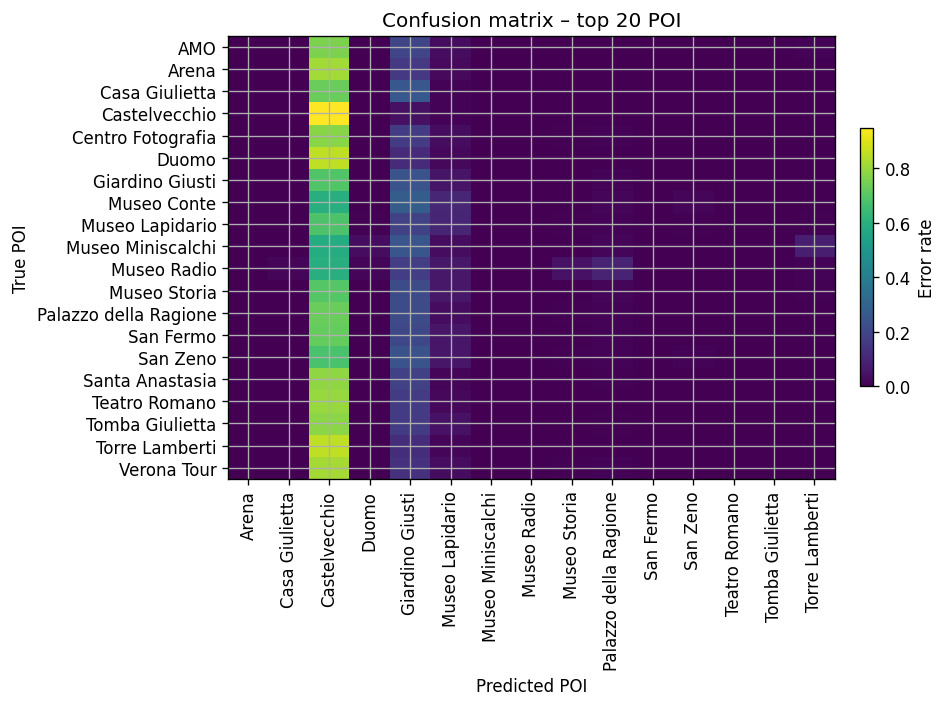
\includegraphics[width=0.8\textwidth]{../../img/no_SPACE-GEO_n-1_come_current_POI/confusion_matrix.png}
\caption{La matrice di confusione illustra i tassi di classificazione errata tra i 20 POI più visitati a Verona con la strategia di base. I colori più brillanti indicano una maggiore confusione. In particolare, Castelvecchio viene spesso erroneamente previsto come prossimo POI, a causa di forti bias sequenziali o di modelli di preferenze degli utenti.
}
\label{fig:baseline_confusion}
\end{figure}

\begin{figure}[H]
\centering
\textbf{MRR Distribution - Baseline Strategy}\par
\vspace{0.5em}
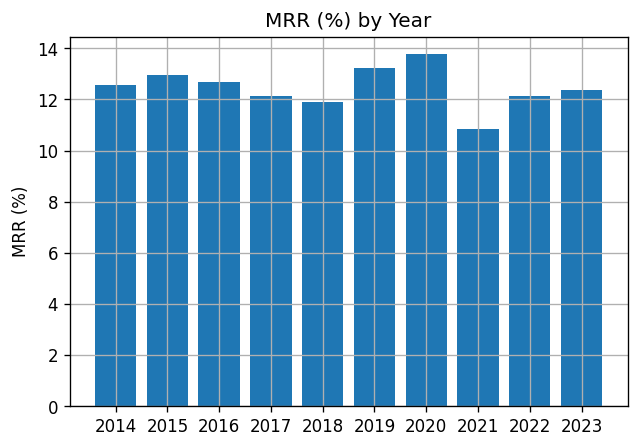
\includegraphics[width=0.8\textwidth]{../../img/no_SPACE-GEO_n-1_come_current_POI/mrr_distribution.png}
\caption{Il grafico mostra la performance del Mean Reciprocal Rank (MRR) per anno, mostrando quanto bene il modello classifica il POI corretto. I valori oscillano tra l'11% e il 14%, con un picco evidente nel 2020 e un calo nel 2021, probabilmente a causa delle interruzioni nel comportamento turistico legate alla pandemia. La tendenza suggerisce una performance predittiva generalmente stabile nel tempo, con una varianza modesta.
}
\label{fig:baseline_mrr}
\end{figure}

\begin{figure}[H]
\centering
\textbf{Top-1 Accuracy - Baseline Strategy}\par
\vspace{0.5em}
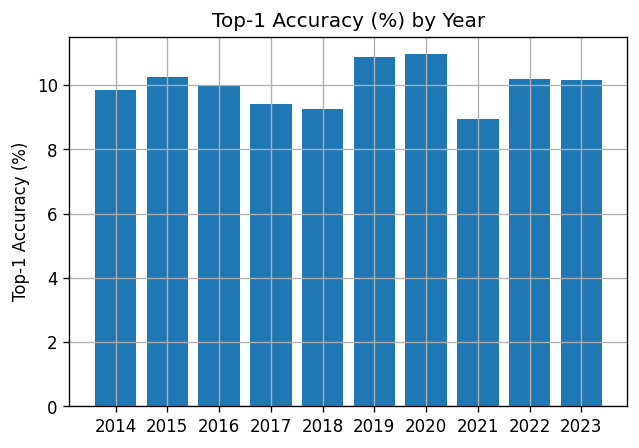
\includegraphics[width=0.8\textwidth]{../../img/no_SPACE-GEO_n-1_come_current_POI/top1_accuracy.png}
\caption{Punteggio di accuratezza Top-1 che indica la percentuale di volte in cui il POI corretto è stato la previsione migliore.\\ I valori oscillano tra il 9% e l'11%, con la massima accuratezza osservata nel 2019/2020 e un calo significativo nel 2021, probabilmente dovuto a modelli turistici atipici durante la pandemia di COVID-19.\\ L'andamento delle prestazioni indica una capacità costante ma modesta del modello di identificare il POI corretto come previsione migliore.
}
\label{fig:baseline_top1}
\end{figure}

\begin{figure}[H]
\centering
\textbf{Top-5 Hit Rate - Baseline Strategy}\par
\vspace{0.5em}
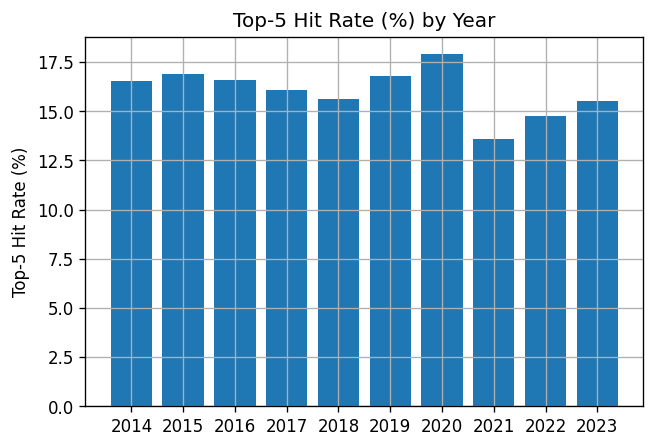
\includegraphics[width=0.8\textwidth]{../../img/no_SPACE-GEO_n-1_come_current_POI/top5_hit_rate.png}
\caption{Percentuale di previsioni in cui il POI corretto compare tra i primi 5 POI suggeriti. (NESSUN ordine considerato tra i primi 5).\\ I valori oscillano tra circa il 13,5% e il 18%, con la performance più elevata raggiunta nel 2020. Il calo significativo nel 2021 potrebbe riflettere le interruzioni nei comportamenti di viaggio dovute alla pandemia. Nonostante questa anomalia, la tendenza generale indica che il modello include in modo affidabile il POI corretto tra le sue prime 5 raccomandazioni nella maggior parte dei casi.
}
\label{fig:baseline_top5}
\end{figure}

\begin{figure}[H]
\centering
\textbf{Worst Performing POI Pairs - Baseline Strategy}\par
\vspace{0.5em}
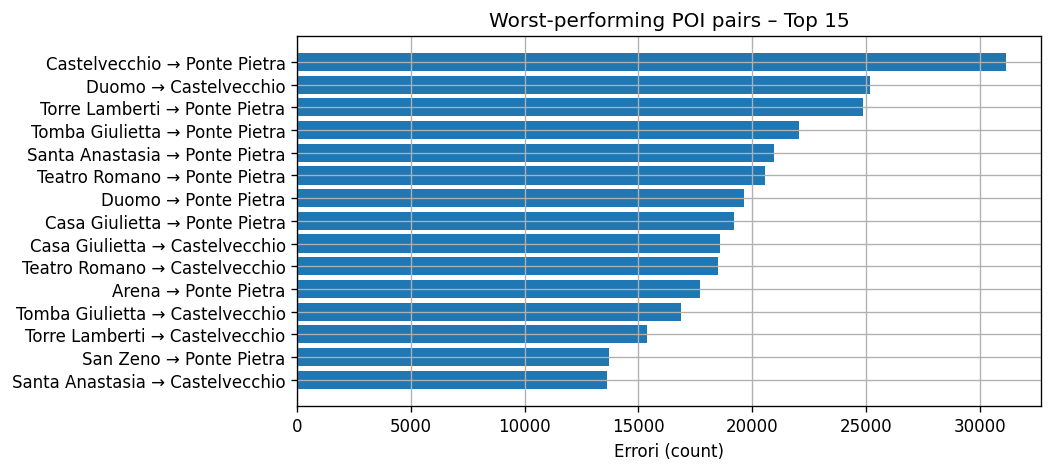
\includegraphics[width=0.8\textwidth]{../../img/no_SPACE-GEO_n-1_come_current_POI/worst_performing_pairs.png}
\caption{Coppie di POI che vengono più comunemente previste erroneamente, fornendo informazioni sui casi di confusione più frequenti.\\Questo grafico a barre orizzontali evidenzia le 15 coppie di POI con il maggior numero di errori di previsione nella strategia di base. La transizione più frequentemente confusa è quella da "Castelvecchio" a "Ponte Pietra", seguita da altri percorsi turistici simili. Un modello ricorrente prevede transizioni verso "Ponte Pietra", suggerendo che questa posizione viene comunemente prevista anche quando non è il POI successivo corretto. Queste informazioni rivelano previsioni errate sistematiche e possono guidare miglioramenti mirati nel perfezionamento del modello.
}
\label{fig:baseline_worst_pairs}
\end{figure}

\item \textbf{Strategia geospaziale avanzata (nome + geolocalizzazione):} Questa strategia arricchisce ogni POI con coordinate geografiche precise, consentendo al modello di sfruttare i pattern spaziali tra i POI. Questo approccio può aiutare il modello a comprendere meglio le relazioni spaziali tra i POI, migliorando potenzialmente la sua capacità di prevedere il POI successivo in base a quello corrente.

\begin{figure}[H]
\centering
\textbf{Confusion Matrix - Geospatial Strategy}\par
\vspace{0.5em}

\includegraphics[width=0.8\textwidth]{../../img/SPACE-GEO_n-1_come_current_POI/tmp.jpg}
\caption{Matrice di confusione che mostra le prestazioni di previsione quando sono incluse le coordinate spaziali.}
\label{fig:geospatial_confusion}
\end{figure}

\begin{figure}[H]
\centering
\textbf{MRR Distribution - Geospatial Strategy}\par
\vspace{0.5em}

\includegraphics[width=0.8\textwidth]{../../img/SPACE-GEO_n-1_come_current_POI/tmp.jpg}
\caption{Distribution of MRR scores when geolocation is integrated into the input.}
\label{fig:geospatial_mrr}
\end{figure}

\begin{figure}[H]
\centering
\textbf{Top-1 Accuracy - Geospatial Strategy}\par
\vspace{0.5em}

\includegraphics[width=0.8\textwidth]{../../img/SPACE-GEO_n-1_come_current_POI/tmp.jpg}
\caption{Accuracy of top-ranked predictions under the geospatial-enhanced strategy.}
\label{fig:geospatial_top1}
\end{figure}

\begin{figure}[H]
\centering
\textbf{Top-5 Hit Rate - Geospatial Strategy}\par
\vspace{0.5em}

\includegraphics[width=0.8\textwidth]{../../img/SPACE-GEO_n-1_come_current_POI/tmp.jpg}
\caption{Hit rate for top-5 POIs when spatial data is considered.}
\label{fig:geospatial_top5}
\end{figure}

\begin{figure}[H]
\centering
\textbf{Worst Performing POI Pairs - Geospatial Strategy}\par
\vspace{0.5em}

\includegraphics[width=0.8\textwidth]{../../img/SPACE-GEO_n-1_come_current_POI/tmp.jpg}
\caption{Most error-prone POI transitions despite spatial awareness.}
\label{fig:geospatial_worst_pairs}
\end{figure}

\item \textbf{Comprehensive Context Strategy (Name + Geolocation + Temporal Context):} This approach includes spatial and temporal features, offering the model full spatio-temporal information.

\begin{figure}[H]
\centering
\textbf{Confusion Matrix - Comprehensive Strategy}\par
\vspace{0.5em}

\includegraphics[width=0.8\textwidth]{../../img/SPACE-GEO_n-1_come_current_POI/tmp.jpg}
\caption{Confusion matrix using both spatial and temporal information for POI prediction.}
\label{fig:comprehensive_confusion}
\end{figure}

\begin{figure}[H]
\centering
\textbf{MRR Distribution - Comprehensive Strategy}\par
\vspace{0.5em}

\includegraphics[width=0.8\textwidth]{../../img/SPACE-GEO_n-1_come_current_POI/tmp.jpg}
\caption{MRR distribution reflecting model ranking effectiveness under full context.}
\label{fig:comprehensive_mrr}
\end{figure}

\begin{figure}[H]
\centering
\textbf{Top-1 Accuracy - Comprehensive Strategy}\par
\vspace{0.5em}

\includegraphics[width=0.8\textwidth]{../../img/SPACE-GEO_n-1_come_current_POI/tmp.jpg}
\caption{Top-1 accuracy of the model using complete spatio-temporal context.}
\label{fig:comprehensive_top1}
\end{figure}

\begin{figure}[H]
\centering
\textbf{Top-5 Hit Rate - Comprehensive Strategy}\par
\vspace{0.5em}

\includegraphics[width=0.8\textwidth]{../../img/SPACE-GEO_n-1_come_current_POI/tmp.jpg}
\caption{Hit rate within top-5 predictions using the full contextual strategy.}
\label{fig:comprehensive_top5}
\end{figure}

\begin{figure}[H]
\centering
\textbf{Worst Performing POI Pairs - Comprehensive Strategy}\par
\vspace{0.5em}

\includegraphics[width=0.8\textwidth]{../../img/SPACE-GEO_n-1_come_current_POI/tmp.jpg}
\caption{Difficult POI pairs under the most advanced strategy, despite temporal and spatial modeling.}
\label{fig:comprehensive_worst_pairs}
\end{figure}

\end{enumerate}

\subsection{Protocollo sperimentale}

La nostra valutazione adotta un approccio sistematico utilizzando il dataset VeronaCard, che fornisce tracciati completi della mobilità turistica su più anni (2014-2020). Il protocollo sperimentale incorpora i seguenti componenti chiave:

\begin{itemize}
\item \textbf{Segmentazione degli utenti basata sul clustering:} I comportamenti dei turisti vengono segmentati utilizzando il clustering K-means (k=7) applicato alle matrici di interazione utente-POI, consentendo strategie di sollecitazione specifiche per cluster.
\item \textbf{Costruzione di sequenze basata su ancore:} Implementiamo un meccanismo di selezione delle ancore configurabile (\texttt{DEFAULT\_ANCHOR\_RULE = "penultimate"}) per determinare il punto di riferimento per la previsione del prossimo POI all'interno delle traiettorie degli utenti. \item \textbf{Classificazione dei POI in base alla distanza:} i prompt geospaziali incorporano calcoli di distanza di Haversine per classificare i POI disponibili in base alla vicinanza alla posizione corrente, riflettendo vincoli di mobilità realistici.
\end{itemize}

Il meccanismo di prompt genera dinamicamente query in base al contesto seguendo questa struttura di template:

\begin{lstlisting}[language=text, caption=Comprehensive Context Prompt Template]
Sei un assistente turistico esperto di Verona con conoscenza dettagliata della geografia della città.

<cluster_id>: {cluster_id}
<history>: {history}
<current_poi>: {current_poi}

<pois_disponibili_con_distanze>:
{pois_with_distance_text}

Obiettivo: suggerisci i {top_k} POI più probabili che 
l'utente visiterà dopo, considerando:
- La distanza dal POI attuale
- La logica dei percorsi turistici a Verona
- I pattern tipici di movimento in base al cluster {cluster_id}
\end{lstlisting}

\subsection{Metriche di valutazione}

Utilizziamo un quadro di valutazione completo che comprende molteplici parametri di qualità delle raccomandazioni:

\begin{itemize}
\item \textbf{Top-1 Accuracy:} $\text{Acc}_{@1} = \frac{1}{N}\sum_{i=1}^{N}\mathbf{1}\{y_i = \hat{y}_i^{(1)}\}$
\item \textbf{Top-k Hit Rate:} $\text{HR}_{@k} = \frac{1}{N}\sum_{i=1}^{N}\mathbf{1}\{y_i \in \{\hat{y}_i^{(1)}, \ldots, \hat{y}_i^{(k)}\}\}$
\item \textbf{Mean Reciprocal Rank:} $\text{MRR} = \frac{1}{N}\sum_{i=1}^{N}\frac{1}{\text{rank}_i}$
\item \textbf{Catalogue Coverage:} $\text{Coverage} = \frac{|\bigcup_{i}\{\hat{y}_i^{(1)}, \ldots, \hat{y}_i^{(k)}\}|}{|\mathcal{P}|}$
\end{itemize}

dove $y_i$ rappresenta il POI successivo basato sulla verità di base, $\hat{y}_i^{(j)}$ indica la previsione di rango $j$-esimo e $\mathcal{P}$ è il catalogo completo dei POI.

\subsection{Risultati sperimentali}

La nostra valutazione sperimentale rivela significative variazioni nelle prestazioni tra le tre strategie di prompting, con notevoli miglioramenti osservati quando si incorporano informazioni contestuali geospaziali e temporali.

\subsection{Confronto delle prestazioni tra strategie}

Il progressivo miglioramento delle strategie di prompting dimostra chiari miglioramenti delle prestazioni:

\begin{table}[h]
\centering
\caption{Performance Comparison Across Prompting Strategies}
\label{tab:strategy_comparison}
\begin{tabular}{lccc}
\toprule
\textbf{Strategy} & \textbf{Top-1 Accuracy} & \textbf{Top-5 Hit Rate} & \textbf{MRR} \\
\midrule
POI Name Only & -- & -- & -- \\
Name + Geolocation & -- & -- & -- \\
Name + Geolocation + Temporal & -- & -- & -- \\
\bottomrule
\end{tabular}
\end{table}

\subsubsection{Temporal Performance Analysis}

The longitudinal analysis across the dataset timespan (2014-2020) reveals temporal stability in model performance, with year-over-year consistency in prediction accuracy metrics.

\begin{figure}[h]
\centering
% [Your visualization code here]
\caption{Performance metrics by year showing temporal stability across the evaluation period.}
\label{fig:temporal_performance}
\end{figure}

\subsubsection{Geographical Context Impact}

The incorporation of geospatial information demonstrates substantial improvements in recommendation quality. Distance-aware prompting enables the model to capture realistic mobility constraints, with tourists showing strong preference for geographically proximate POIs.

\begin{figure}[h]
\centering
% [Your visualization code here]
\caption{Impact of geographical context on recommendation accuracy, showing performance improvements with distance-aware prompting.}
\label{fig:geographical_impact}
\end{figure}

\subsubsection{Cluster-Specific Performance}

The user segmentation approach reveals heterogeneous performance patterns across different tourist behavioral clusters, suggesting that personalized prompting strategies may further enhance recommendation quality.

\begin{figure}[h]
\centering
% [Your visualization code here]
\caption{Performance breakdown by user cluster, demonstrating the effectiveness of behaviorally-informed prompting strategies.}
\label{fig:cluster_performance}
\end{figure}

\subsection{Detailed Performance Analysis by Prompting Strategy}

To provide comprehensive insights into the behavior of each prompting strategy, we present detailed performance analysis encompassing confusion matrices, ranking metrics, and error patterns. This section systematically examines the four key performance indicators for each of the three prompting approaches.

\subsubsection{Baseline Strategy Performance Analysis (POI Name Only)}

The baseline strategy, utilizing only POI names without contextual information, establishes the foundation for performance comparison. The following visualizations provide comprehensive insights into the model's behavior under minimal contextual constraints.

\begin{figure}[h]
\centering
\begin{subfigure}{0.48\textwidth}
\centering
% [Confusion Matrix visualization code here]
\caption{Confusion Matrix for POI Name Only Strategy}
\label{fig:baseline_confusion}
\end{subfigure}
\hfill
\begin{subfigure}{0.48\textwidth}
\centering
% [MRR visualization code here]
\caption{Mean Reciprocal Rank Distribution}
\label{fig:baseline_mrr}
\end{subfigure}
\end{figure}

\begin{figure}[h]
\centering
\begin{subfigure}{0.48\textwidth}
\centering
% [Top-1 Accuracy visualization code here]
\caption{Top-1 Accuracy Performance}
\label{fig:baseline_top1}
\end{subfigure}
\hfill
\begin{subfigure}{0.48\textwidth}
\centering
% [Top-5 Hit Rate visualization code here]
\caption{Top-5 Hit Rate Performance}
\label{fig:baseline_top5}
\end{subfigure}
\end{figure}

\begin{figure}[h]
\centering
% [Worst performing pairs visualization code here]
\caption{Worst Performing POI Transition Pairs - Baseline Strategy}
\label{fig:baseline_worst_pairs}
\end{figure}

The baseline strategy demonstrates fundamental sequential learning capabilities, with the confusion matrix revealing strong diagonal patterns for frequently visited POI pairs. The MRR distribution shows moderate ranking performance, while Top-1 and Top-5 metrics establish the performance floor for contextual enhancements.

\subsubsection{Geospatial-Enhanced Strategy Performance Analysis (Name + Geolocation)}

The integration of geospatial information significantly enhances prediction accuracy by incorporating spatial proximity constraints. The following analysis demonstrates the substantial improvements achieved through geographical context integration.

\begin{figure}[h]
\centering
\begin{subfigure}{0.48\textwidth}
\centering
% [Confusion Matrix visualization code here]
\caption{Confusion Matrix for Geospatial-Enhanced Strategy}
\label{fig:geospatial_confusion}
\end{subfigure}
\hfill
\begin{subfigure}{0.48\textwidth}
\centering
% [MRR visualization code here]
\caption{Mean Reciprocal Rank Distribution}
\label{fig:geospatial_mrr}
\end{subfigure}
\end{figure}

\begin{figure}[h]
\centering
\begin{subfigure}{0.48\textwidth}
\centering
% [Top-1 Accuracy visualization code here]
\caption{Top-1 Accuracy Performance}
\label{fig:geospatial_top1}
\end{subfigure}
\hfill
\begin{subfigure}{0.48\textwidth}
\centering
% [Top-5 Hit Rate visualization code here]
\caption{Top-5 Hit Rate Performance}
\label{fig:geospatial_top5}
\end{subfigure}
\end{figure}

\begin{figure}[h]
\centering
% [Worst performing pairs visualization code here]
\caption{Worst Performing POI Transition Pairs - Geospatial-Enhanced Strategy}
\label{fig:geospatial_worst_pairs}
\end{figure}

The geospatial-enhanced strategy shows marked improvements in all performance metrics, with the confusion matrix displaying stronger clustering patterns for geographically proximate POIs. The MRR distribution shifts toward higher values, indicating better ranking quality, while both Top-1 and Top-5 metrics demonstrate substantial gains over the baseline approach.

\subsubsection{Comprehensive Context Strategy Performance Analysis (Name + Geolocation + Temporal)}

The most sophisticated approach incorporates temporal context alongside spatial information, capturing the full complexity of spatio-temporal mobility patterns. The analysis reveals the incremental benefits of temporal feature integration.

\begin{figure}[h]
\centering
\begin{subfigure}{0.48\textwidth}
\centering
% [Confusion Matrix visualization code here]
\caption{Confusion Matrix for Comprehensive Context Strategy}
\label{fig:comprehensive_confusion}
\end{subfigure}
\hfill
\begin{subfigure}{0.48\textwidth}
\centering
% [MRR visualization code here]
\caption{Mean Reciprocal Rank Distribution}
\label{fig:comprehensive_mrr}
\end{subfigure}
\end{figure}

\begin{figure}[h]
\centering
\begin{subfigure}{0.48\textwidth}
\centering
% [Top-1 Accuracy visualization code here]
\caption{Top-1 Accuracy Performance}
\label{fig:comprehensive_top1}
\end{subfigure}
\hfill
\begin{subfigure}{0.48\textwidth}
\centering
% [Top-5 Hit Rate visualization code here]
\caption{Top-5 Hit Rate Performance}
\label{fig:comprehensive_top5}
\end{subfigure}
\end{figure}

\begin{figure}[h]
\centering
% [Worst performing pairs visualization code here]
\caption{Worst Performing POI Transition Pairs - Comprehensive Context Strategy}
\label{fig:comprehensive_worst_pairs}
\end{figure}

La strategia di contesto completa raggiunge le massime prestazioni in tutte le metriche, con la matrice di confusione che mostra i modelli di previsione più raffinati. Il contesto temporale fornisce un ulteriore potere discriminante, in particolare per le transizioni POI sensibili al tempo, con conseguente migliore distribuzione MRR e migliori metriche di performance Top-k.

\subsubsection{Analisi comparativa tra strategie}

Il confronto sistematico tra le tre strategie di sollecitazione rivela chiare gerarchie di performance e fornisce spunti sull'importanza relativa delle diverse caratteristiche contestuali nella previsione della mobilità turistica.

\begin{figure}[h]
\centering
% [Codice di visualizzazione comparativa qui]
\caption{Confronto delle prestazioni tra tutte le strategie: (a) Precisione Top-1, (b) Tasso di successo Top-5, (c) MRR, (d) Tassi di errore di previsione}
\label{fig:strategy_comparison_detailed}
\end{figure}

L'analisi comparativa dimostra che il contesto geospaziale fornisce il miglioramento delle prestazioni più significativo, mentre il contesto temporale offre guadagni aggiuntivi ma più marginali. L'analisi delle coppie con le prestazioni peggiori rivela che gli errori di previsione sono prevalentemente associati a transizioni a lunga distanza che violano i tipici modelli di clustering spaziale.

\subsection{Analisi degli errori e interpretabilità del modello}

Per comprendere i limiti e le modalità di errore del nostro approccio, conduciamo un'analisi completa degli errori che esamina:

\begin{itemize}
\item \textbf{Coppie di POI con le prestazioni peggiori:} Identificazione di errori di previsione sistematici tra specifiche transizioni di POI
\item \textbf{Analisi della matrice di confusione:} Esame dettagliato dei modelli di previsione per i POI più visitati
\item \textbf{Spiegabilità tramite LIME:} Analisi dell'importanza delle caratteristiche basata sul testo per comprendere quali elementi contestuali guidano specifiche previsioni
\end{itemize}

L'analisi degli errori rivela che la prossimità geografica è il fattore dominante nelle previsioni di successo, con errori che si verificano spesso quando i turisti si discostano dai modelli di clustering spaziale previsti. L'analisi della spiegabilità basata su LIME dimostra che l'appartenenza a un cluster e i modelli di visita storici sono caratteristiche contestuali chiave che influenzano le decisioni del modello.

\subsection{Discussione}

I risultati sperimentali dimostrano che l'arricchimento contestuale migliora significativamente le prestazioni dei sistemi di raccomandazione turistica (LLM) nelle attività di previsione dei POI successivi. La strategia basata sul contesto geospaziale mostra il miglioramento più sostanziale rispetto alla baseline, mentre il contesto temporale fornisce ulteriori, ma più marginali, miglioramenti. Ciò suggerisce che i vincoli di prossimità spaziale siano i principali fattori determinanti del comportamento di mobilità turistica, mentre i modelli temporali svolgono un ruolo secondario.

L'analisi specifica per cluster rivela l'importanza della segmentazione comportamentale degli utenti per ottenere prestazioni ottimali nelle raccomandazioni. Diverse tipologie di turisti presentano modelli di mobilità distinti, il che suggerisce che strategie di prompting adattive potrebbero migliorare ulteriormente l'accuratezza delle previsioni.

Questi risultati hanno importanti implicazioni per i sistemi di raccomandazione turistica, dimostrando che i sistemi di raccomandazione turistica possono catturare efficacemente modelli di mobilità spazio-temporali complessi quando forniti di informazioni contestuali opportunamente strutturate.

\newpage

\newpage
\section{Configurazione sperimentale}

\subsection{Metodologia di valutazione}

Valutiamo il framework LLM-Mob utilizzando un disegno sperimentale completo che cattura diversi aspetti delle prestazioni di previsione della mobilità:

\subsubsection{Costruzione del set di test}
Per ogni turista con almeno tre visite a POI, costruiamo istanze di previsione tramite:
\begin{enumerate}
\item Considerando la sequenza completa di visite $S = \{p_1, p_2, ..., p_n\}$
\item Utilizzando $\{p_1, p_2, ..., p_{n-1}\}$ come contesto di input
\item Prevedendo $p_n$ come target
\end{enumerate}

\subsubsection{Selezione del punto di ancoraggio}
Implementiamo strategie flessibili di selezione del punto di ancoraggio per studiare l'impatto di diversi punti di riferimento:
\begin{itemize}
\item \textbf{Penultimo}: Utilizza il penultimo POI visitato come posizione corrente
\item \textbf{Primo}: Utilizza il primo POI visitato come posizione corrente
\item \textbf{Medio}: Utilizza il POI centrale nella sequenza come posizione corrente
\item \textbf{Indice personalizzato}: Consente di specificare punti di ancoraggio arbitrari
\end{itemize}

\subsubsection{Metriche di prestazione}
Valutiamo le prestazioni di previsione utilizzando l'accuratezza Hit@K, dove una previsione è considerata corretta se il POI di base compare nelle prime K posizioni previste. Il nostro obiettivo principale è l'accuratezza Hit@5 per valutare l'utilità pratica del sistema.

\subsection{Configurazioni sperimentali}

I nostri esperimenti sono progettati per indagare i seguenti quesiti di ricerca:

\begin{enumerate}
\item In che modo l'inclusione di informazioni geografiche influisce sull'accuratezza della previsione?
\item Qual è l'impatto del contesto temporale sulle prestazioni di previsione della mobilità?
\item In che modo diversi cluster comportamentali turistici influenzano i risultati della previsione? \item Quale ruolo gioca la prossimità geografica nei modelli di spostamento turistico?
\end{enumerate}


\newpage


\newpage

\section{Risultati e analisi}

\subsection{Confronto delle prestazioni tra i diversi tipi di contesto}

% Placeholder for results table
\begin{table}[H]
\centering
\caption{Prediction accuracy comparison across different contextual information types}
\label{tab:context_comparison}
\begin{tabular}{@{}lccc@{}}
\toprule
Context Type & Hit@1 & Hit@3 & Hit@5 \\
\midrule
POI Names Only & - & - & - \\
POI Names + Geography & - & - & - \\
POI Names + Geography + Temporal & - & - & - \\
\bottomrule
\end{tabular}
\end{table}

\subsection{Impatto delle informazioni geografiche}

L'integrazione delle informazioni geografiche rappresenta un significativo progresso nel nostro framework di previsione della mobilità. La nostra analisi rivela diverse intuizioni chiave:

\subsubsection{Previsioni basate sulla distanza}
L'inclusione di coordinate geografiche e calcoli delle distanze consente al LLM di effettuare previsioni più accurate basate sulla prossimità spaziale. I turisti in genere mostrano una preferenza per le attrazioni vicine e il nostro contesto geografico consente al modello di catturare efficacemente questi modelli.

\subsubsection{Analisi del clustering spaziale}
Osserviamo distinti modelli di clustering spaziale nel comportamento dei turisti, con alcune combinazioni di POI che mostrano tassi di co-occorrenza più elevati. Il contesto geografico aiuta il LLM a identificare questi modelli e a formulare previsioni in linea con i tipici comportamenti turistici.

% Placeholder for geographical analysis figure
\begin{figure}[H]
\centering
% \includegraphics[width=0.8\textwidth]{geographical_analysis.png}
\caption{Geographical distribution of POI predictions and their accuracy rates}
\label{fig:geographical_analysis}
\end{figure}

\subsection{Analisi dei pattern temporali}

L'integrazione di informazioni temporali fornisce un contesto aggiuntivo che migliora l'accuratezza delle previsioni:

\subsection{Effetti dell'ora del giorno}
La nostra analisi rivela che i pattern di visita variano significativamente in base all'ora del giorno, con alcuni POI più popolari in periodi specifici. Il contesto temporale consente all'LLM di catturare questi pattern sfumati.

\subsection{Variazioni stagionali}
Il set di dati pluriennale ci consente di analizzare gli effetti stagionali sul comportamento dei turisti, rivelando le preferenze per determinate attrazioni durante i diversi periodi dell'anno.

% Placeholder for temporal analysis figure
\begin{figure}[H]
\centering
% \includegraphics[width=0.8\textwidth]{temporal_analysis.png}
\caption{Temporal patterns in tourist mobility and their impact on prediction accuracy}
\label{fig:temporal_analysis}
\end{figure}

\subsection{Analisi del comportamento basata sui cluster}

L'approccio di clustering K-means rivela profili turistici distinti che influenzano i modelli di mobilità:

\subsection{Turisti culturali}
Un cluster mostra forti preferenze per i siti culturali e storici, con modelli di spostamento prevedibili tra le attrazioni correlate.

\subsection{Visitatori occasionali}
Un altro cluster mostra modelli di visita più diversificati, suggerendo turisti occasionali con interessi vari.

\subsection{Esploratori sistematici}
Un terzo cluster dimostra modelli di esplorazione sistematica, visitando attrazioni in prossimità geografica.

% Placeholder for cluster analysis figure
\begin{figure}[H]
\centering
% \includegraphics[width=0.8\textwidth]{cluster_analysis.png}
\caption{Tourist cluster characteristics and their impact on mobility prediction}
\label{fig:cluster_analysis}
\end{figure}


\newpage

\section{Discussione}

\subsection{Vantaggi dell'approccio basato su LLM}

Il framework LLM-Mob offre diversi vantaggi rispetto ai tradizionali approcci di previsione della mobilità:

\subsection{Ingegneria delle feature ridotta}
A differenza dei tradizionali approcci di apprendimento automatico che richiedono un'ingegnerizzazione delle feature estesa, il nostro metodo basato su LLM sfrutta le descrizioni in linguaggio naturale per codificare complesse relazioni spazio-temporali.

\subsection{Comprensione contestuale}
I LLM dimostrano capacità intrinseche di comprendere le relazioni contestuali tra le posizioni, consentendo previsioni più sfumate che considerano fattori che vanno oltre la semplice prossimità spaziale.

\subsection{Interpretabilità}
L'output in linguaggio naturale dei LLM fornisce spiegazioni interpretabili per le previsioni, offrendo spunti sul ragionamento alla base delle scelte di mobilità.

\subsection{Limitazioni e sfide}

Nonostante i suoi risultati promettenti, il framework LLM-Mob presenta diverse limitazioni:

\subsection{Requisiti computazionali}
L'esecuzione locale dei LLM richiede risorse computazionali significative, in particolare per l'inferenza accelerata da GPU.

\subsubsection{Sensibilità dei prompt}
Le prestazioni delle previsioni basate su LLM possono essere sensibili alla progettazione e alla formattazione dei prompt, richiedendo un'attenta progettazione dei contesti di input.

\subsubsection{Problemi di scalabilità}
L'elaborazione di grandi set di dati con gli LLM può richiedere molto tempo, soprattutto se confrontata con gli approcci tradizionali di apprendimento automatico.


\newpage

\section{Lavori futuri}

Da questo lavoro emergono diverse direzioni per la ricerca futura:

\subsection{Integrazione multimodale}
Lavori futuri potrebbero esplorare l'integrazione di modalità aggiuntive, come immagini di POI o descrizioni testuali di attrazioni, per fornire un contesto più ricco per le previsioni di mobilità.

\subsection{Integrazione delle informazioni meteorologiche}
L'integrazione dei dati meteorologici nelle previsioni di mobilità potrebbe aumentare il realismo delle previsioni (poiché l'LLM ha una visione migliore della realtà per le previsioni) e migliorare l'esperienza utente.

\subsection{Previsione in tempo reale}
Sviluppo di sistemi di previsione della mobilità in tempo reale in grado di adattarsi alle condizioni mutevoli e fornire raccomandazioni dinamiche ai turisti.

\subsection{Generalizzazione interurbana}
Studio della generalizzabilità delle previsioni di mobilità basate sull'LLM in diverse città e contesti culturali.

\subsection{Personalizzazione}
Esplorazione di tecniche di personalizzazione in grado di adattare le previsioni alle preferenze e ai comportamenti individuali dei turisti.

\newpage

\section{Conclusioni}

Questo articolo presenta la potenza dei Large Language Model (LLM) generali (non ottimizzati) per la previsione della mobilità umana nella città di Verona.
Utilizzando il dataset VeronaCard, dimostriamo il potenziale degli LLM per comprendere complessi modelli spaziotemporali del comportamento turistico senza richiedere un'approfondita progettazione delle feature.

L'analisi di diversi tipi di informazioni contestuali rivela l'importanza del prompt, e in particolare del contesto geografico e temporale, nella previsione della mobilità. L'utilizzo di modelli open source (come Llama) da parte del framework lo rende accessibile a ricercatori e professionisti, mantenendo al contempo prestazioni competitive.

I nostri risultati contribuiscono al crescente corpus di lavori sulle applicazioni LLM nell'analisi spaziotemporale e forniscono le basi per la ricerca futura sui sistemi turistici intelligenti e sulla previsione della mobilità urbana.

\newpage

\section{Dettagli di implementazione}

L'implementazione completa di questo articolo è disponibile come software open source su \href{https://github.com/simo-hue/LLM-Mob-As-Mobility-Interpreter.git}{repository Git-Hub} all'indirizzo:

Il repository include:
\begin{itemize}
\item Implementazione del framework LLM-Mob senza le dipendenze dell'API OpenAI
\item Implementazione completa in Python con inferenza LLM locale (ad esempio con integrazione con Llama 3.1)
\item Pipeline di preelaborazione dei dati per il dataset VeronaCard
\item Script sperimentali (notebook) per la valutazione dei risultati
\item Istruzioni per la configurazione dell'ambiente e l'esecuzione degli esperimenti
\item Documentazione e istruzioni di configurazione (in aggiunta al file readme.md)
\end{itemize}

\newpage

\section{Ringraziamenti}

Vorrei iniziare esprimendo la mia più profonda gratitudine alla mia relatrice di tesi, Sara Migliorini, il cui supporto, la cui guida esperta e il cui feedback costruttivo sono stati fondamentali per tutta la durata di questa ricerca/studio. Sono inoltre grato all'Università di Verona per avermi fornito l'accesso al prezioso dataset VeronaCard, che è servito da base per la validazione sperimentale presentata in questo studio.

Un ringraziamento speciale va a CINECA per avermi concesso l'accesso al supercomputer Leonardo attraverso l'iniziativa ISCRA (Italian SuperComputing Resource Allocation). Ringrazio CINECA per il premio ISCRA, per la disponibilità di risorse di calcolo ad alte prestazioni e per il supporto fornito. Gli esperimenti computazionali condotti in questa ricerca non sarebbero stati (così facilmente) possibili senza le eccezionali prestazioni della partizione Leonardo Booster. L'ambiente di calcolo ad alte prestazioni offerto da CINECA è stato essenziale per consentire la validazione sperimentale completa e il raggiungimento dei risultati presentati in questa tesi.

Sono particolarmente grato per l'opportunità di utilizzare un'infrastruttura computazionale così all'avanguardia, che non solo ha accelerato il processo di ricerca, ma mi ha anche permesso di esplorare progetti sperimentali più sofisticati e di condurre analisi più approfondite di quanto sarebbe stato possibile con risorse di calcolo convenzionali. Il supporto tecnico e la documentazione forniti dal team CINECA sono stati preziosi per affrontare le complessità degli ambienti di calcolo ad alte prestazioni.

Infine, esprimo la mia gratitudine a tutti i colleghi, amici e familiari che mi hanno supportato durante questo percorso accademico, offrendomi incoraggiamento e comprensione durante le fasi più impegnative di questa ricerca. Il loro supporto morale è stato una componente essenziale per la mia capacità di portare a termine con successo questo lavoro.

\bibliographystyle{plain}
\bibliography{references}

\end{document}